% Matching games: eliciting preferences, then running Gale-Shapley by hand.
% Shared preamble for the write-on class slides.
%
% Every deck is designed to be projected and annotated live on a tablet:
% whatever takes time to draw is pre-drawn, and whatever the class produces is
% left blank. Compile a deck with `pdflatex main.tex` from its own directory,
% or run `make` in decks/ to build them all.
\documentclass[10pt]{article}

\usepackage[papersize={25.6cm,14.4cm}, margin=1.1cm, bottom=1.5cm,
            footskip=0.75cm]{geometry}
\usepackage[T1]{fontenc}
\usepackage[default]{sourcesanspro}
\usepackage{newtxsf}
\usepackage{tikz}
\usepackage{amsmath}
\usepackage{parskip}
\usepackage{fancyhdr}
\usetikzlibrary{arrows.meta, positioning, calc}

\setlength{\parindent}{0pt}

% Catppuccin Latte, the palette the course site uses in its light theme, so a
% deck on the projector looks like the pages the students read.
\definecolor{inkbg}{HTML}{EFF1F5}      % base
\definecolor{inksurface}{HTML}{E6E9EF} % mantle
\definecolor{inkfaint}{HTML}{CCD0DA}   % surface2, for rules and empty boxes
\definecolor{inktext}{HTML}{4C4F69}    % text
\definecolor{inkgrey}{HTML}{8C8FA1}    % overlay1, for anything secondary
\definecolor{inkblue}{HTML}{7287FD}    % lavender, the primary accent
\definecolor{inkteal}{HTML}{179299}    % teal
\definecolor{inkred}{HTML}{FE640B}     % peach, for whatever wants attention
\definecolor{inkmauve}{HTML}{8839EF}   % mauve

\pagecolor{inkbg}
\color{inktext}

% A box to write a number into. White against the tinted page, so it reads as
% somewhere to write rather than as part of the printed material.
\newcommand{\blank}[1][1.6]{%
  \tikz[baseline=(current bounding box.base)]{%
    \draw[inkfaint, line width=0.7pt, rounded corners=2pt, fill=white]
      (0,-0.18) rectangle (#1,0.62);}}

% A ruled area to work in. Faint dots keep handwriting level on a tablet.
\newcommand{\workspace}[2]{%
  \begin{tikzpicture}
    \draw[inkfaint, line width=0.7pt, rounded corners=3pt, fill=white]
      (0,0) rectangle (#1,#2);
    \foreach \gx in {0.5,1.0,...,#1}{%
      \foreach \gy in {0.5,1.0,...,#2}{%
        \fill[inkfaint] (\gx,\gy) circle (0.5pt);}}
  \end{tikzpicture}}

% A panel for material that is printed rather than written on.
\newcommand{\panel}[2]{%
  \begin{tikzpicture}
    \draw[inkfaint, line width=0.7pt, rounded corners=3pt, fill=inksurface]
      (0,0) rectangle (#1,#2);
  \end{tikzpicture}}

% An empty payoff grid. #1 is the list of action names, #2 is drawn afterwards
% so a page can add its own marks.
\newcommand{\payoffgrid}[2]{%
  \begin{tikzpicture}[scale=1.0, every node/.style={transform shape}]
    \foreach \name [count=\j from 0] in {#1}{%
      \node[font=\bfseries, text=inkblue] at (\j*2.7+1.35,0.55) {\name};
      \node[font=\bfseries, text=inkblue] at (-1.15,-\j*2-1) {\name};
      \foreach \k [count=\i from 0] in {#1}{%
        \draw[inkfaint, line width=0.7pt, fill=white]
          (\j*2.7,-\i*2) rectangle (\j*2.7+2.7,-\i*2-2);}}
    #2
  \end{tikzpicture}}

% The five actions on a pentagon. Each action beats the one next to it and the
% one across from it, so the two winning cycles are drawn as separate panels:
% ten labelled arrows on one diagram is a tangle nobody can read from the back
% of the room.
\newcommand{\rpslscycle}[3]{%
  \begin{tikzpicture}[scale=1.0, every node/.style={transform shape},
      >={Stealth[length=2.6mm]},
      action/.style={circle, draw=inkfaint, line width=1pt, fill=white,
                     text=inktext, minimum size=1.7cm, inner sep=1pt,
                     font=\small\bfseries},
      beats/.style={->, line width=1.2pt, shorten >=3pt, shorten <=3pt,
                    draw=#1},
      word/.style={font=\scriptsize, fill=inkbg, inner sep=1.6pt, text=#1,
                   sloped, pos=#2}]
    \foreach \name/\angle in {Rock/90, Lizard/18, Spock/-54,
                              Scissors/-126, Paper/162}{%
      \node[action] (\name) at (\angle:3.1) {\name};}
    \foreach \winner/\loser/\said in {#3}{%
      \draw[beats] (\winner) -- node[word] {\said} (\loser);}
  \end{tikzpicture}}

% Running header: the deck name on the left, the page's own step on the right.
% Each deck sets its name once with \deckname.
\newcommand{\deck}{}
\newcommand{\deckname}[1]{\renewcommand{\deck}{#1}}
\newcommand{\slidehead}[1]{%
  {\small\color{inkgrey}%
   \tikz[baseline=-0.5ex]{\fill[inkblue, rounded corners=1pt]
     (0,0) rectangle (0.22,0.22);}\;\deck
   \hfill \color{inkblue}\bfseries #1}\par
  {\color{inkblue}\rule{\linewidth}{1pt}}\par\vspace{0.35em}}

\pagestyle{fancy}
\fancyhf{}
\renewcommand{\headrulewidth}{0pt}
\fancyfoot[R]{\small\color{inkgrey}\thepage}

% Deck title pages, which carry no header and no page number.
\newcommand{\titleslide}[3]{%
  \thispagestyle{empty}%
  \begin{center}
    \vspace*{\fill}
    {\Huge\bfseries\color{inkblue} #1}\\[0.7em]
    {\LARGE\color{inkgrey} #2}\\[2.4em]
    #3
    \vspace*{\fill}
  \end{center}}

% One step of the plan on a title page.
\newcommand{\stepbox}[3]{%
  \node[draw=inkblue, line width=0.9pt, rounded corners=4pt, fill=white,
        minimum width=6cm, minimum height=1.7cm, align=center,
        text=inktext] (#1) at (#2,0) {#3};}


% The two sides of the market, with #1 drawn afterwards so each round can add
% its own proposals, holds and rejections.
\newcommand{\bipartite}[1]{%
  \begin{tikzpicture}[scale=1.5, every node/.style={transform shape},
      person/.style={draw=inkblue, line width=0.9pt, fill=white, text=inkblue,
                     rounded corners=3pt, minimum width=2.3cm,
                     minimum height=0.72cm, font=\small\bfseries}]
    \foreach \name [count=\i from 0] in {Gauss, Noether, Turing, Euler}{%
      \node[person] (m\i) at (0,-\i*1.25) {\name};}
    \foreach \name [count=\i from 0] in {Einstein, Curie, Newton, Feynman}{%
      \node[person, draw=inkteal, text=inkteal] (p\i) at (4.7,-\i*1.25)
        {\name};}
    #1
  \end{tikzpicture}}

% One person's preference list, waiting to be filled in.
\newcommand{\prefrow}[1]{%
  \makebox[2.1cm][l]{#1}
  \blank[2]\, \blank[2]\, \blank[2]\, \blank[2]}

\deckname{Matching games}

\begin{document}

\titleslide{Matching games}{Four mathematicians, four physicists, one stable matching}{%
    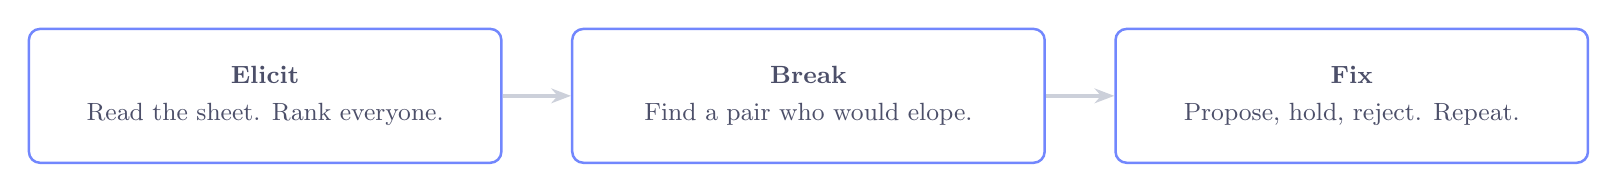
\begin{tikzpicture}[font=\small]
      \stepbox{s0}{0.0}{\textbf{Elicit}\\[0.25em] Read the sheet. Rank everyone.}
      \stepbox{s1}{6.9}{\textbf{Break}\\[0.25em] Find a pair who would elope.}
      \stepbox{s2}{13.8}{\textbf{Fix}\\[0.25em] Propose, hold, reject. Repeat.}
      \draw[-{Stealth[length=2.5mm]}, inkfaint, line width=1.2pt] (s0) -- (s1);
      \draw[-{Stealth[length=2.5mm]}, inkfaint, line width=1.2pt] (s1) -- (s2);
    \end{tikzpicture}}

\newpage
\slidehead{What the groups decided}

\vspace{0.6cm}

\begin{minipage}[t]{0.48\linewidth}
{\large\bfseries\color{inkblue} Mathematicians}

\vspace{0.8em}

{\large
\prefrow{Gauss}\\[1.1em]
\prefrow{Noether}\\[1.1em]
\prefrow{Turing}\\[1.1em]
\prefrow{Euler}}
\end{minipage}
\hfill
\begin{minipage}[t]{0.48\linewidth}
{\large\bfseries\color{inkteal} Physicists}

\vspace{0.8em}

{\large
\prefrow{Einstein}\\[1.1em]
\prefrow{Curie}\\[1.1em]
\prefrow{Newton}\\[1.1em]
\prefrow{Feynman}}
\end{minipage}

\vspace{1.4cm}

{\small\color{inkgrey} Most preferred first. These come from the preference
sheet, not from me.}

\newpage
\slidehead{When is a matching no good?}

\vspace{0.6cm}

{\large Pair everyone up however you like:}

\vspace{0.5cm}

\begin{center}
{\large
\blank[2.6] \; with \; \blank[2.6] \hspace{2.4cm}
\blank[2.6] \; with \; \blank[2.6]\\[1.3em]
\blank[2.6] \; with \; \blank[2.6] \hspace{2.4cm}
\blank[2.6] \; with \; \blank[2.6]}
\end{center}

\vspace{1cm}

{\large Now find two people who would both rather have each other. That pair
is a \underline{\hspace{3.4cm}}, and the matching is
\underline{\hspace{3cm}}.}

\vspace{0.9cm}

\begin{center}
\workspace{22.6}{2.8}
\end{center}

\newpage
\slidehead{Deferred acceptance: rounds 1 and 2}

\vspace{0.2cm}

\begin{minipage}[t]{0.48\linewidth}
\begin{center}
{\large\bfseries Round 1}\\[0.4em]
\bipartite{}
\end{center}
\end{minipage}
\hfill
\begin{minipage}[t]{0.48\linewidth}
\begin{center}
{\large\bfseries Round 2}\\[0.4em]
\bipartite{}
\end{center}
\end{minipage}

\vspace{0.5cm}

{\small\color{inkgrey} Draw each proposal as an arrow. Circle the one held, and
cross out the rejections.}

\newpage
\slidehead{Deferred acceptance: rounds 3 and 4}

\vspace{0.2cm}

\begin{minipage}[t]{0.48\linewidth}
\begin{center}
{\large\bfseries Round 3}\\[0.4em]
\bipartite{}
\end{center}
\end{minipage}
\hfill
\begin{minipage}[t]{0.48\linewidth}
\begin{center}
{\large\bfseries Round 4}\\[0.4em]
\bipartite{}
\end{center}
\end{minipage}

\vspace{0.5cm}

{\small\color{inkgrey} Stop when nobody is left holding a proposal they have not
accepted.}

\newpage
\slidehead{The matching, and why it holds}

\vspace{0.7cm}

\begin{center}
{\large
\blank[2.6] \; with \; \blank[2.6] \hspace{2.4cm}
\blank[2.6] \; with \; \blank[2.6]\\[1.3em]
\blank[2.6] \; with \; \blank[2.6] \hspace{2.4cm}
\blank[2.6] \; with \; \blank[2.6]}
\end{center}

\vspace{1.1cm}

{\large Check it: take any pair who are \emph{not} matched to each other, and
show at least one of them prefers who they have.}

\vspace{0.7cm}

\begin{center}
\workspace{22.6}{3.4}
\end{center}

\vspace{0.4cm}

{\large Who does better out of this, the proposers or the proposed to?
\blank[4]}

\newpage
\slidehead{The same thing, as an exam answer}

\vspace{0.5cm}

{\large What we just did in the room is \textbf{Question 1} on the Matching
Games page, with three on each side instead of four.}

\vspace{0.9cm}

\hspace{0.6cm}
\begin{minipage}{0.92\linewidth}
{\large
\begin{tabbing}
\hspace{1.2cm} \= \hspace{17cm} \= \kill
\textbf{(a)} \> Define a blocking pair and a stable matching, and write the
  preferences as maps. \> [5]\\[0.55em]
\textbf{(b)} \> Run Gale-Shapley with the mathematicians proposing, showing
  each step. \> [7]\\[0.55em]
\textbf{(c)} \> Write down the resulting matching. \> [3]\\[0.55em]
\textbf{(d)} \> Verify it is stable by checking for a blocking pair. \> [4]\\[0.55em]
\textbf{(e)} \> Whose optimum is it, and why can the proposing side never do
  better? \> [6]
\end{tabbing}}
\end{minipage}

\vspace{1.2cm}

\begin{center}
{\large\color{inkgrey} vknight.org/gt/topics/matching-games.html}
\end{center}

\end{document}
